\section{Introduction}

Before introduce how to write a good introduction, I want first emphasize the important of introduction section as below (for the details, see the slides in ``Slides'' folder of this project):

Spend some time to pick a good title for your paper!!! If your paper later has 1000 hundred of readers, 1000 will read your title, 100 read abstract, 100 read introduction, 10 read your problem definition, 10 read related work, maybe just 10 or less than 10 will read your solutions and only 5 read the details of your solution at the end.


Usually, you should write the introduction section two times! 1) Write it first: tell a clear story; 2) write it last: make sure it is telling what you really do in your finished paper.

Here is a good structure for introduction section:

Paragraph 1: Context. What is the background? At most 4 sentences please!

Paragraph 2: Problem area. Some related studies. What is the problem in this area? Don't tell too detailed about the related studies, which is what ``Related Work'' will do.  About 3 sentences are enough.

Paragraph 3-4: What you do in this paper? What is the key point of this paper? You can have a motivation example to show your niche! Usually, people can understand example better than what you explained. Better to draw an interesting figure for you problem. Like the example \cite{cheng2016task} below:

\begin{figure}[h!]\centering
	\scalebox{0.7}[0.7]{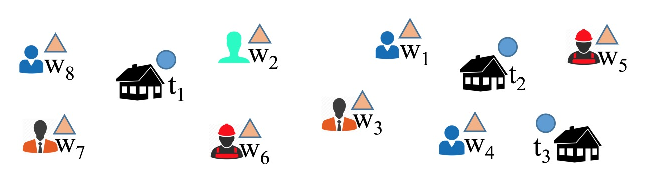
\includegraphics{../figures/motivation_example.eps}}
	\caption{\small An Example of Motivation Example.}
	\label{fig:bbq_example}
\end{figure}

Paragraph 5: challenges in this novel problem. Why it is hard? Why existing solutions cannot solve it?

Paragraph 6: What you have done on solving it?  Similar to the introduction, but more details. Brief summary of results.

Paragraph 7: Outline of this paper. You can modify the example below:

To summarize, we make the following contributions in the paper:
\begin{itemize}[leftmargin=*]
	\item We propose a XXXX problem and prove it is NP-hard in Section \ref{sec:problemDefinition}.\itemMargin
	\item  We proposed solution1 and solution2 in Section \ref{sec:solution1} and \ref{sec:solution2}, respectively.\itemMargin
	\item We have  conducted extensive experiments on real and synthetic data sets, to show the efficiency and effectiveness of our XXX framework/algorithm in Section \ref{sec:experimental}.\itemMargin
\end{itemize}

In addition, the remaining sections of the paper are arranged as
follows. We review and compare previous studies on queueing theory and vehicle dispatching in Section \ref{sec:related} and conclude the work in Section \ref{sec:conclusion}.

